%!TEX TS-program = xelatex
\documentclass[notes,12pt, aspectratio=169]{beamer}

\usepackage{amsmath,amsfonts,amssymb,amsthm,mathtools}  % пакеты для математики
%\usepackage{minted}

\usepackage[english, russian]{babel} % выбор языка для документа
\usepackage[utf8]{inputenc} % задание utf8 кодировки исходного tex файла
\usepackage[X2,T2A]{fontenc}        % кодировка

\usepackage{fontspec}         % пакет для подгрузки шрифтов
\setmainfont{Georgia}  % задаёт основной шрифт документа

% why do we need \newfontfamily:
% http://tex.stackexchange.com/questions/91507/
\newfontfamily{\cyrillicfonttt}{Georgia}
\newfontfamily{\cyrillicfont}{Georgia}
\newfontfamily{\cyrillicfontsf}{Georgia}

\usepackage{unicode-math}     % пакет для установки математического шрифта
% \setmathfont{Neo Euler} % шрифт для математики

\usepackage{polyglossia}      % Пакет, который позволяет подгружать русские буквы
\setdefaultlanguage{russian}  % Основной язык документа
\setotherlanguage{english}    % Второстепенный язык документа

% Шрифт для кода
\setmonofont[Scale=0.85]{Georgia}
\usepackage{verbments}

\usepackage{pgfpages}
% These slides also contain speaker notes. You can print just the slides,
% just the notes, or both, depending on the setting below. Comment out the want
% you want.
%\setbeameroption{hide notes} % Only slide
%\setbeameroption{show only notes} % Only notes
%\setbeameroption{show notes on second screen=right} % Both

\usepackage{array}

\usepackage{tikz}
\usepackage{verbatim}
\setbeamertemplate{note page}{\pagecolor{yellow!5}\insertnote}
\usetikzlibrary{positioning}
\usetikzlibrary{snakes}
\usetikzlibrary{calc}
\usetikzlibrary{arrows}
\usetikzlibrary{decorations.markings}
\usetikzlibrary{shapes.misc}
\usetikzlibrary{matrix,shapes,arrows,fit,tikzmark}

\usepackage{hyperref}
\usepackage{lipsum}
\usepackage{multimedia}
\usepackage{multirow}
\usepackage{dcolumn}
\usepackage{bbm}
\newcolumntype{d}[0]{D{.}{.}{5}}

\usepackage{changepage}
\usepackage{appendixnumberbeamer}
\newcommand{\beginbackup}{
	\newcounter{framenumbervorappendix}
	\setcounter{framenumbervorappendix}{\value{framenumber}}
	\setbeamertemplate{footline}
	{
		\leavevmode%
		\hline
		box{%
			\begin{beamercolorbox}[wd=\paperwidth,ht=2.25ex,dp=1ex,right]{footlinecolor}%
				%         \insertframenumber  \hspace*{2ex} 
		\end{beamercolorbox}}%
		\vskip0pt%
	}
}
\newcommand{\backupend}{
	\addtocounter{framenumbervorappendix}{-\value{framenumber}}
	\addtocounter{framenumber}{\value{framenumbervorappendix}} 
}

% для имитации питоновского синтаксиса 
\newcommand{\pgr}[1]{{\color{green} \textbf{#1}}}


%%%%%%%%%% Работа с картинками %%%%%%%%%
\usepackage{graphicx}                  % Для вставки рисунков
\usepackage{graphics}
\graphicspath{{images/}}    % можно указать папки с картинками
\usepackage{wrapfig}                   % Обтекание рисунков и таблиц текстом

\usepackage[space]{grffile}
\usepackage{booktabs}

% These are my colors -- there are many like them, but these ones are mine.
\definecolor{blue}{RGB}{0,114,178}
\definecolor{red}{RGB}{213,94,0}
\definecolor{yellow}{RGB}{240,228,66}
\definecolor{green}{RGB}{0,128, 0}

\hypersetup{
	colorlinks=false,
	linkbordercolor = {white},
	linkcolor = {blue}
}


%% I use a beige off white for my background
\definecolor{MyBackground}{RGB}{255,253,218}

%% Uncomment this if you want to change the background color to something else
%\setbeamercolor{background canvas}{bg=MyBackground}

%% Change the bg color to adjust your transition slide background color!
\newenvironment{transitionframe}{
	\setbeamercolor{background canvas}{bg=yellow}
	\begin{frame}}{
\end{frame}
}

\setbeamercolor{frametitle}{fg=blue}
\setbeamercolor{title}{fg=black}
\setbeamertemplate{footline}[frame number]
\setbeamertemplate{navigation symbols}{} 
\setbeamertemplate{itemize items}{-}
\setbeamercolor{itemize item}{fg=blue}
\setbeamercolor{itemize subitem}{fg=blue}
\setbeamercolor{enumerate item}{fg=blue}
\setbeamercolor{enumerate subitem}{fg=blue}
\setbeamercolor{button}{bg=MyBackground,fg=blue,}
\usepackage{hyperref}
\usepackage{graphicx}

% If you like road maps, rather than having clutter at the top, have a roadmap show up at the end of each section 
% (and after your introduction)
% Uncomment this is if you want the roadmap!
% \AtBeginSection[]
% {
%    \begin{frame}
%        \frametitle{Roadmap of Talk}
%        \tableofcontents[currentsection]
%    \end{frame}
% }
\setbeamercolor{section in toc}{fg=blue}
\setbeamercolor{subsection in toc}{fg=red}
\setbeamersize{text margin left=1em,text margin right=1em} 

% списки, которые растягиваются на всю величину слайда 
\newenvironment{wideitemize}{\itemize\addtolength{\itemsep}{10pt}}{\enditemize}



\title[]{\textcolor{blue}{Глубокое обучение и вообще}}
\author{Ульянкин Филипп}
\date{\today}


\begin{document}

%%% TIKZ STUFF
\tikzset{   
        every picture/.style={remember picture,baseline},
        every node/.style={anchor=base,align=center,outer sep=1.5pt},
        every path/.style={thick},
        }
\newcommand\marktopleft[1]{%
    \tikz[overlay,remember picture] 
        \node (marker-#1-a) at (-.3em,.3em) {};%
}
\newcommand\markbottomright[2]{%
    \tikz[overlay,remember picture] 
        \node (marker-#1-b) at (0em,0em) {};%
}
\tikzstyle{every picture}+=[remember picture] 
\tikzstyle{mybox} =[draw=black, very thick, rectangle, inner sep=10pt, inner ysep=20pt]
\tikzstyle{fancytitle} =[draw=black,fill=red, text=white]
%%%% END TIKZ STUFF

% Title Slide
\begin{frame}
\maketitle
\centering \textbf{\color{blue} Посиделка 16:} Улица Сезам
\end{frame}


\begin{frame}{Agenda} 
\begin{wideitemize}
	\item  Развитие идеи эмбедингов
	\item  Seq2seq модели
	\item  История автоперевода
	\item  RNN и механизм внимания
	\item  Attention is all you need
	\item  Модификации трансформера
\end{wideitemize}
\end{frame}


\begin{transitionframe}
	\begin{center}
		\Huge  Развитие идеи эмбедингов
	\end{center}
\end{transitionframe}


\begin{frame}{Серия вопросов в зал}
\begin{wideitemize}
	\item Как работают разные эмбединги?
	\item В чем, по вашему мнению, их главная проблема?
\end{wideitemize}
\end{frame}


\begin{frame}{Embedings from language models (ELMO)}
\begin{center}
	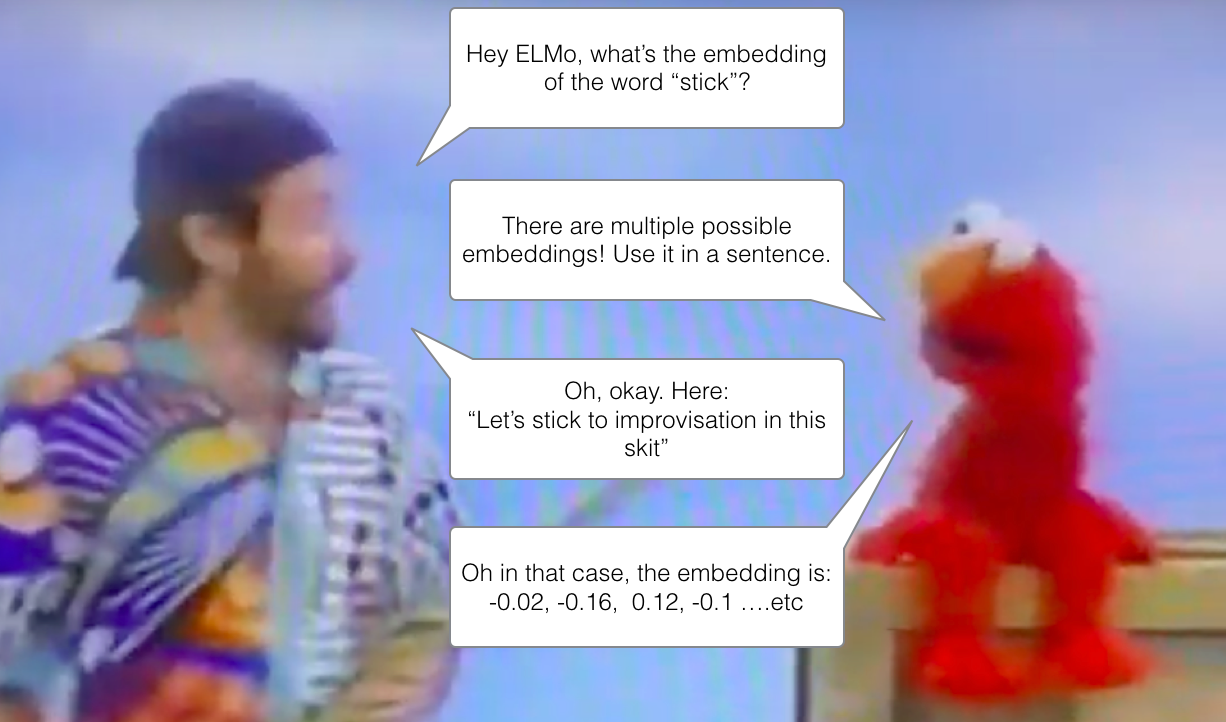
\includegraphics[width=0.9\linewidth]{elmo-embedding-robin-williams}
\end{center}
\end{frame}


\begin{frame}{ELMO}
\begin{center}
	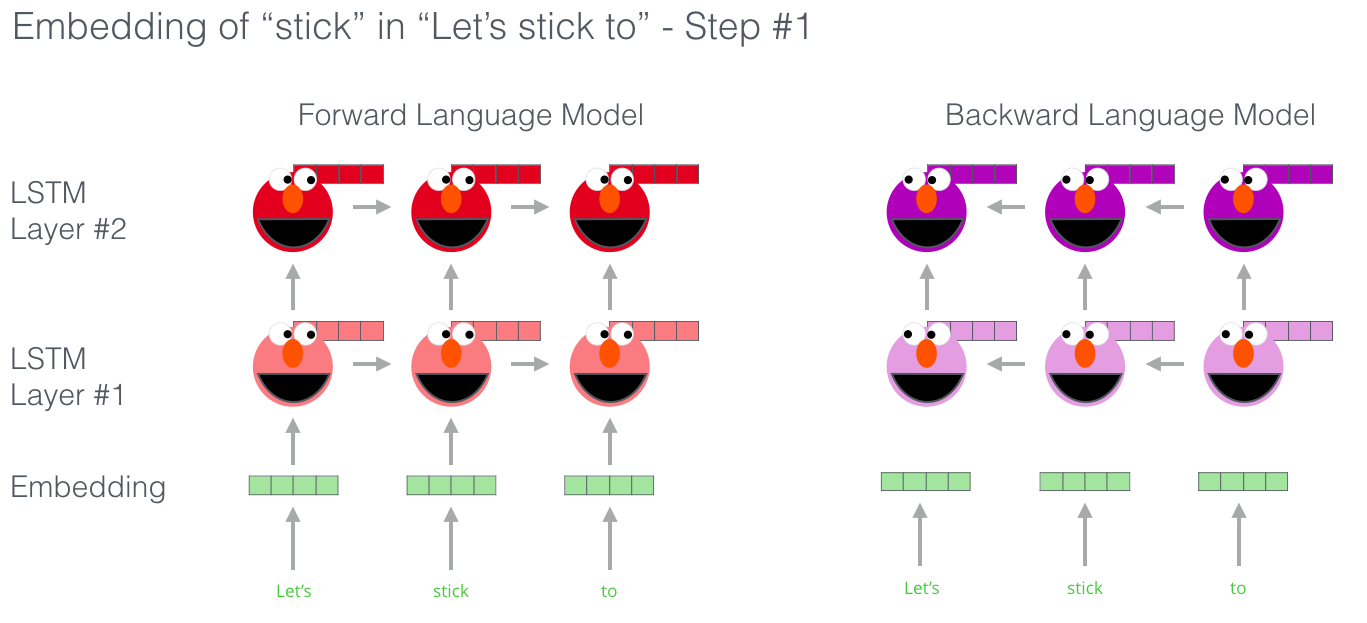
\includegraphics[width=0.9\linewidth]{elmo_model.png}
\end{center}
\vfill
\footnotesize
{\color{blue} \url{http://jalammar.github.io/illustrated-bert/}}
\end{frame}


\begin{frame}{ELMO}
\begin{wideitemize}
	\item Захватываем контекст предложения через biderictional LSTM 
	\item Модель пытается предсказать следующее слово в предложении 
\end{wideitemize}
\vfill
\footnotesize
{\color{blue} \url{https://arxiv.org/pdf/1802.05365.pdf}}
\end{frame}


\begin{frame}{ELMO}
	В качестве эмбединга используется вектор  $[T, h^l, h^r]$, где $T$ - токены, которые сетка выплёвывает наружу, $h_l$ - итоговое скрытое состояние ячеек при проходе слева направо, $h^r$- справа налево.
	
	\begin{center}
		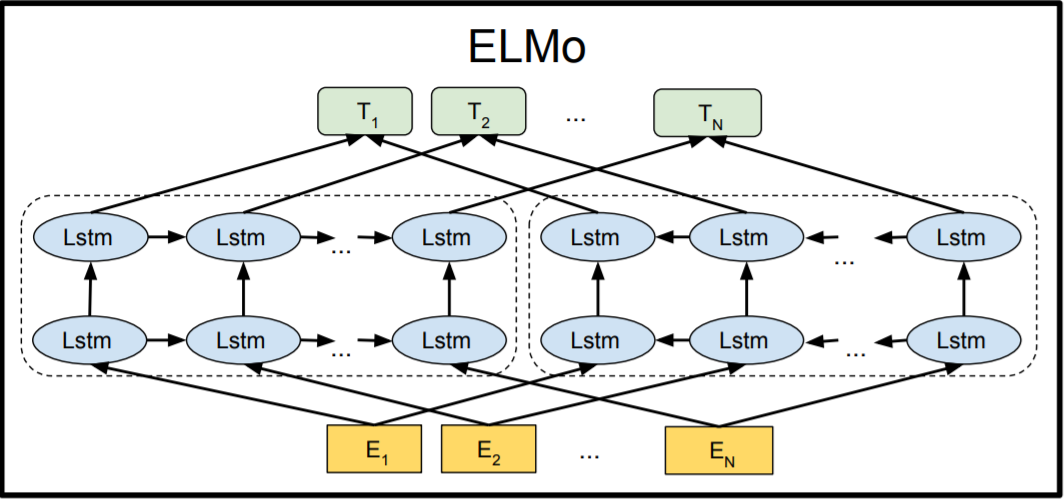
\includegraphics[width=0.7\linewidth]{elmo.png}
	\end{center}
	
	\vfill
	\footnotesize
	{\color{blue} \url{https://arxiv.org/pdf/1802.05365.pdf}}
\end{frame}


\begin{transitionframe}
	\begin{center}
		\Huge RNN и механизм внимания
	\end{center}
\end{transitionframe}


\begin{frame}{Проблема RNN} 
\begin{wideitemize}
	\item  При решении seq2seq задач предложения произвольной длины кодируются в вектор фиксированного размера 
	\item  В длинных предложениях теряется контекст, длинные предложения не зависят от начальных токенов
	\item LSTM и BiLSTM пытаются частично решить эту проблему
\end{wideitemize}

\vfill
\begin{center}
	
\includegraphics[width=.98\linewidth]{translate.jpg}
\end{center}
\end{frame}


\begin{frame}{Автопереводы} 
	\begin{center}
		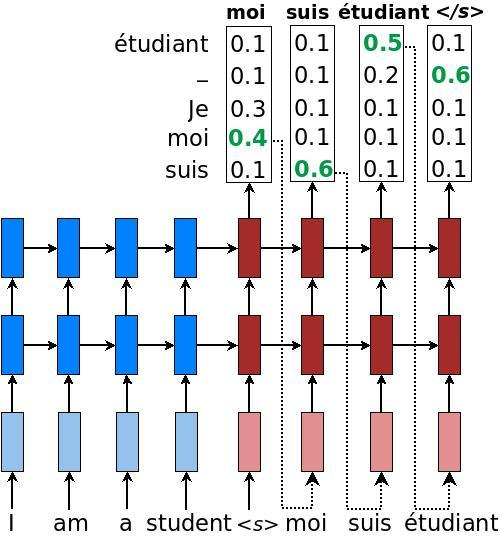
\includegraphics[width=.42\linewidth]{greedy_dec.jpg}
	\end{center}

\vfill
\footnotesize
{\color{blue} \url{https://github.com/tensorflow/nmt}}
\end{frame}


\begin{frame}{Проблемы seq2seq архитектуры} 
\begin{wideitemize}
	\item  Нужно сжать весь текст в один вектор
	\item  Теряется информация о первых словах
	\item  Декодер тоже может терять информацию по мере генерации
	последовательности
	\item  Можно использовать BiLSTM, но тогда будет теряться
	информация о словах в середине
\end{wideitemize}
\end{frame}


\begin{frame}{Механизм внимания} 
\begin{columns}[T] %
	\begin{column}{.35\textwidth}
		\centering
		\resizebox{0.8\linewidth}{!}{
			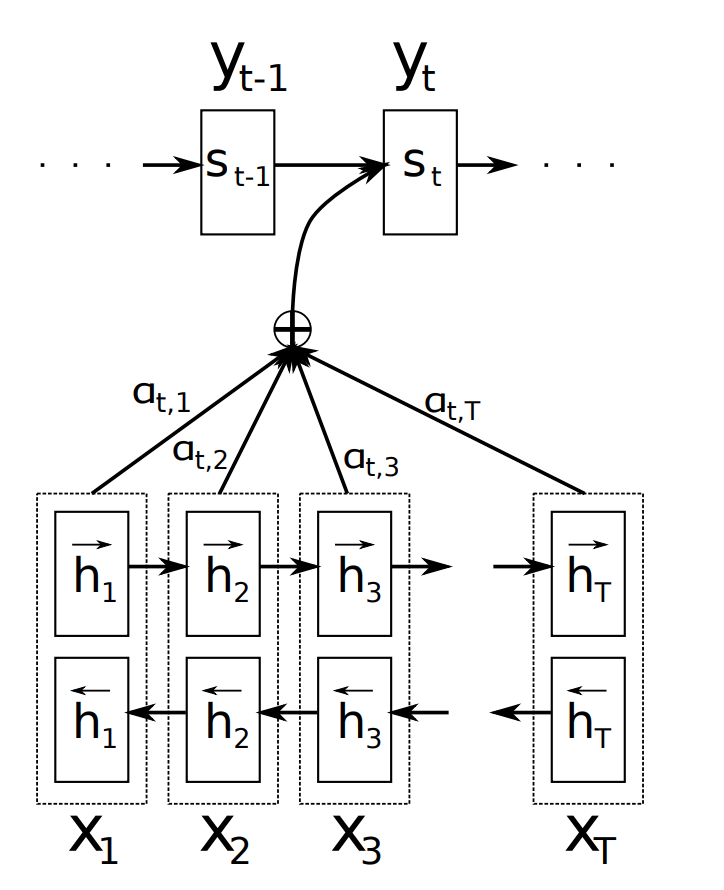
\includegraphics{attention01.png}
		}
	
	\vfill
	\scriptsize
	{\color{blue} \url{https://arxiv.org/pdf/1409.0473.pdf}}
	\end{column}%
	\hfill%
	\begin{column}{.65\textwidth}
		\only<1>{
		\begin{wideitemize}
			\item На вход энкодеру подаём все скрытые состояния 
			\item Хотим научить нейросеть смотреть в нужные места исходной последовательности
		\end{wideitemize}}
	\only<2>{ 
		\begin{itemize}
			\item Скрытое состояние декодировщика $$h_t^d = g(\hat{y}_{t-1}, h_{t-1}^d, c_t)$$
			\item Релевантность $i$-го входного слова $t$-ому (обычно это полносвязный слой): $$sim(h_j^e, h_{t-1}^d) $$
			\item Распределение на входных словах: $$ \alpha_{it} = Softmax(sim(h_j^e, h_{t-1}^d))) $$
			\item  Пытаюсь угадать какие слова входной последовательности важны:  $ c_t = \sum_i \alpha_{jt} \cdot h_j^e $			
		\end{itemize}}
	\end{column}%
\end{columns}
\end{frame}


\begin{frame}{Механизм внимания} 
\begin{center}
	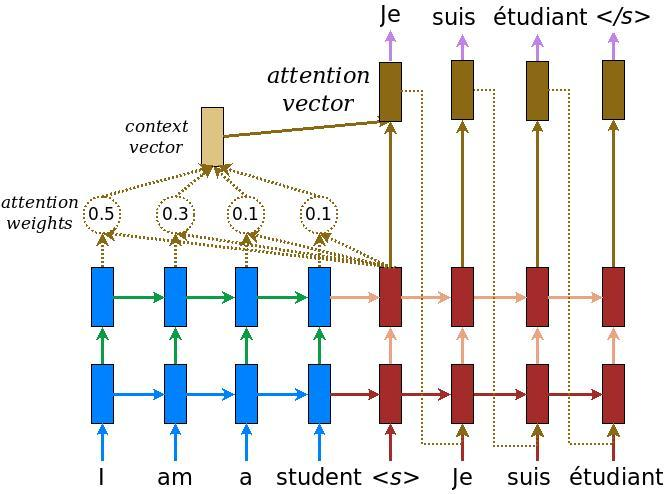
\includegraphics[width=.6\linewidth]{attention_mechanism.jpg}
\end{center}
\vfill
\footnotesize
{\color{blue} \url{https://github.com/tensorflow/nmt}}
\end{frame}


\begin{frame}{Механизм внимания}
\begin{center}
	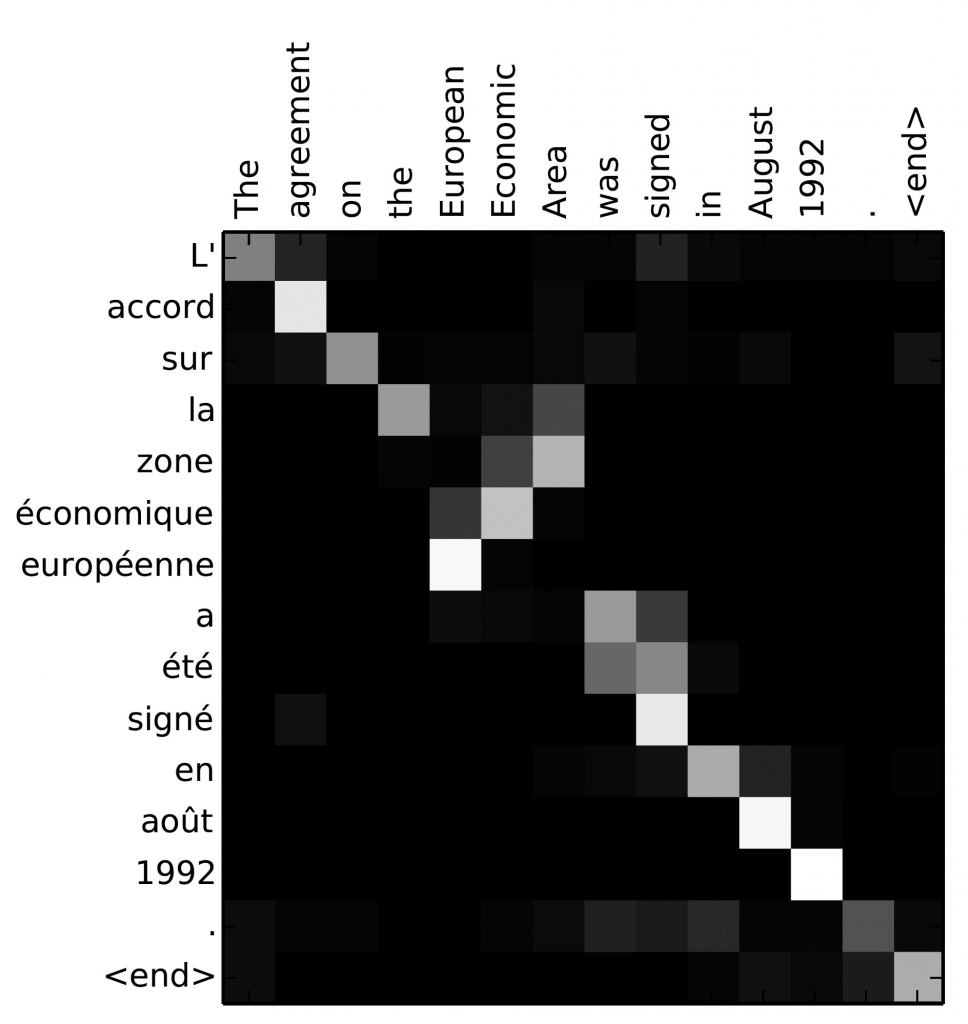
\includegraphics[width=0.47\linewidth]{undestend_attention}
\end{center}
\end{frame}


\begin{frame}{Как посчитать sim?} 
\begin{wideitemize}
	\item  Скалярное произведение: $$sim(h,s) = h^T\cdot s$$
	\item  Additive attention:  $$sim(h,s) = W^T \cdot tanh(W_hh+W_ss )$$	
	\item  Multiplicative attention: $$sim(h,s) = h^TWs$$	
	\item  $W, W_s, W_h$ - обучаемые параметры
	\item Многие-многие другие функции из разных модных работ :)
\end{wideitemize}
\end{frame}


\begin{transitionframe}
	\begin{center}
		\Huge Как сделать seq2seq быстрее без потери качества?
	\end{center}
\end{transitionframe}


\begin{frame}{Attention is All You Need! (2017)} 
\begin{wideitemize}
	\item  RNN это очень долго! Всегда, чтобы найти следующий токен, надо знать предыдущий 
	\item  Backward pass идёт ещё и через время :(
	\item  Transformer — нейросетевая архитектура для задач seq2seq, основанная
	исключительно на полносвязных слоях
	\item Превзошла существовавшие seq2seq архитектуры как по качеству, так и по скорости
	работы
	\item Основной элемент — multi-head self-attention
\end{wideitemize}
\end{frame}


\begin{frame}{Transformer} 

\alert{Верхнеуровнего - это просто энкодер и декодер}

\begin{center}
	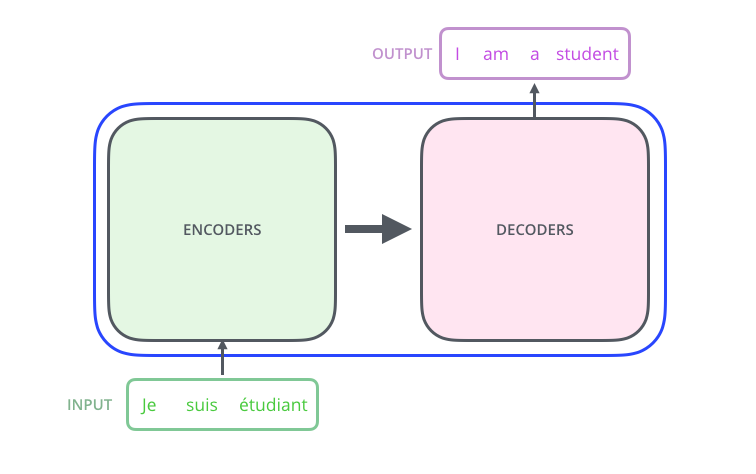
\includegraphics[width=.6\linewidth]{transformer01.png}
\end{center}
\vfill
\footnotesize
{\color{blue} \url{http://jalammar.github.io/illustrated-transformer/}}
\end{frame}


\begin{frame}{Transformer} 

Энкодер и декодер состоят из одинаковых блоков; веса во всех блоках разные

\begin{center}
	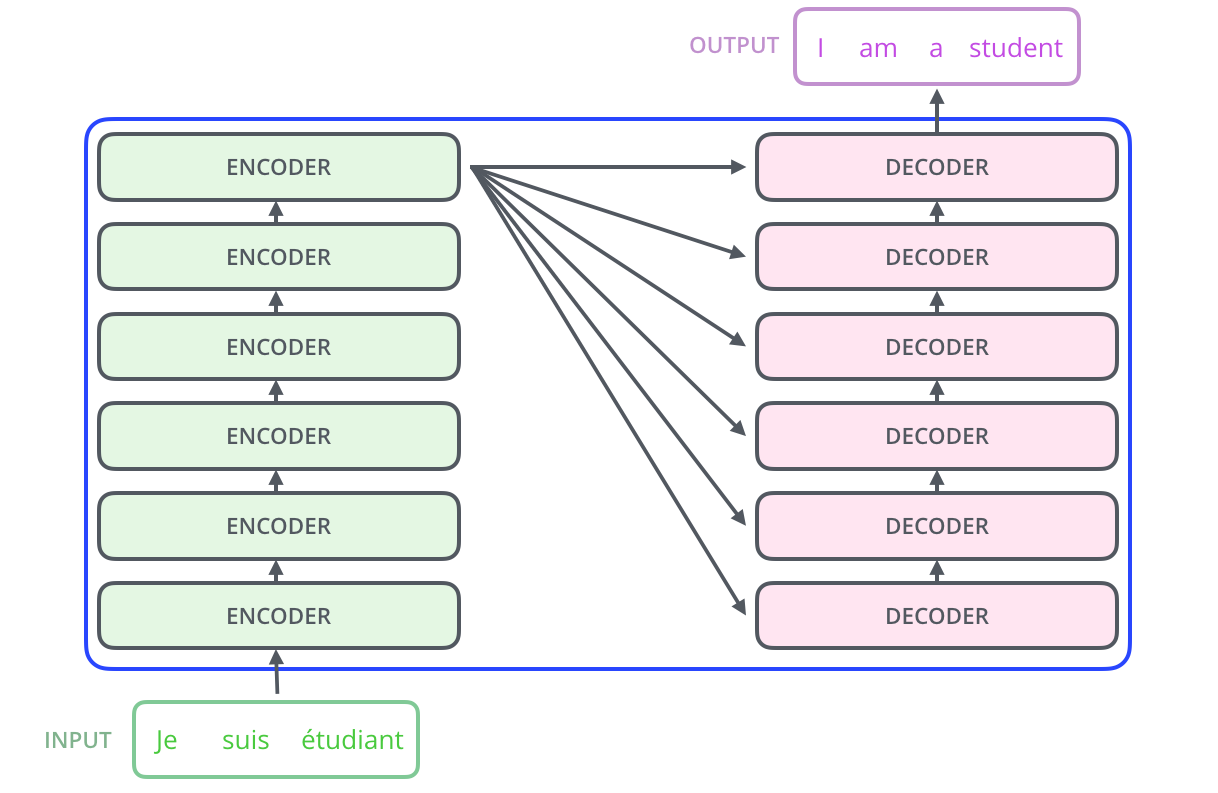
\includegraphics[width=.6\linewidth]{transformer02.png}
\end{center}
\vfill
\footnotesize
{\color{blue} \url{http://jalammar.github.io/illustrated-transformer/}}
\end{frame}


\begin{frame}{Transformer} 

В энкодере происходят две вещи: сначала вход прогоняется через self-attention, а затем —
через полносвязный слой. В декодере помимо обычного self-attention есть ещё и attention
из энкодера.

\begin{center}
	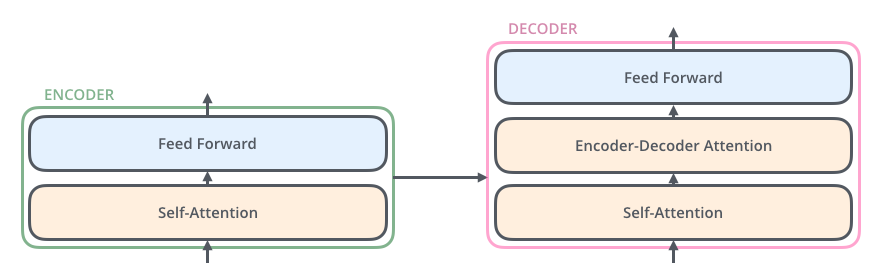
\includegraphics[width=.8\linewidth]{tranformer03.png}
\end{center}
\vfill
\footnotesize
{\color{blue} \url{http://jalammar.github.io/illustrated-transformer/}}
\end{frame}


\begin{frame}{Self-attention} 
\begin{center}
	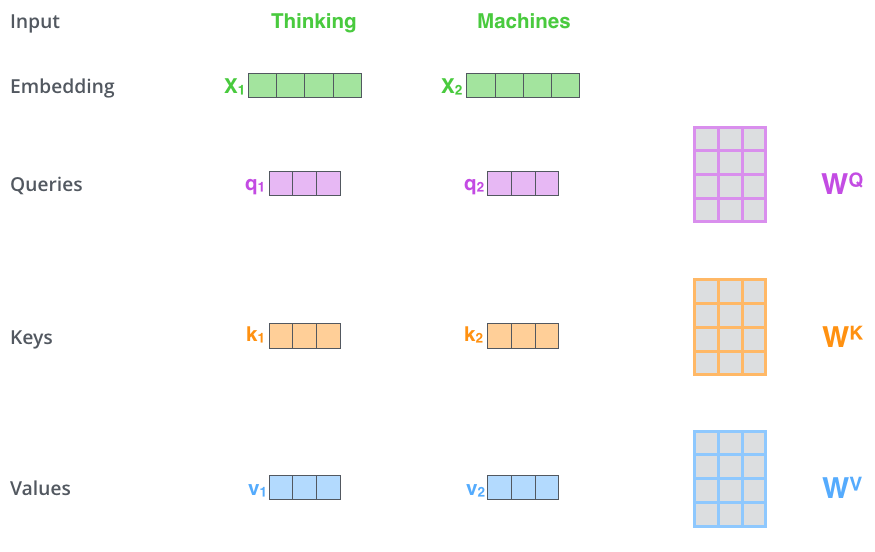
\includegraphics[width=.7\linewidth]{selfattention.png}
\end{center}
\end{frame}


\begin{frame}{Абстракции}
\begin{wideitemize}
	\item  Для каждого входного слова считаются три вектора: Query, Key и Value
	\item  Матрицы $W^Q, W^K , W^V$ обучаются вместе с моделью
	\item  Value - то, что мы знаем об этом слове
	\item  Query, Key помогают искать связи между словами, мы ходим по всем словам и пытаемся понять насколько они связаны между собой 
	\item Query - мое текущее слово, Key - мое слово с которым я сравниваю себя
\end{wideitemize}
\end{frame}


\begin{frame}{Self-attention} 
Цель этого слоя — сложить Value с некоторыми весами

\begin{center}
	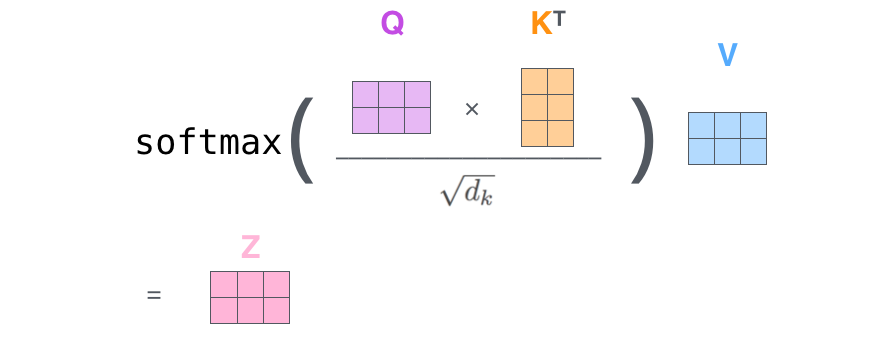
\includegraphics[width=.9\linewidth]{self_final.png}
\end{center}
\end{frame}


\begin{frame}{Более детально}
\centering
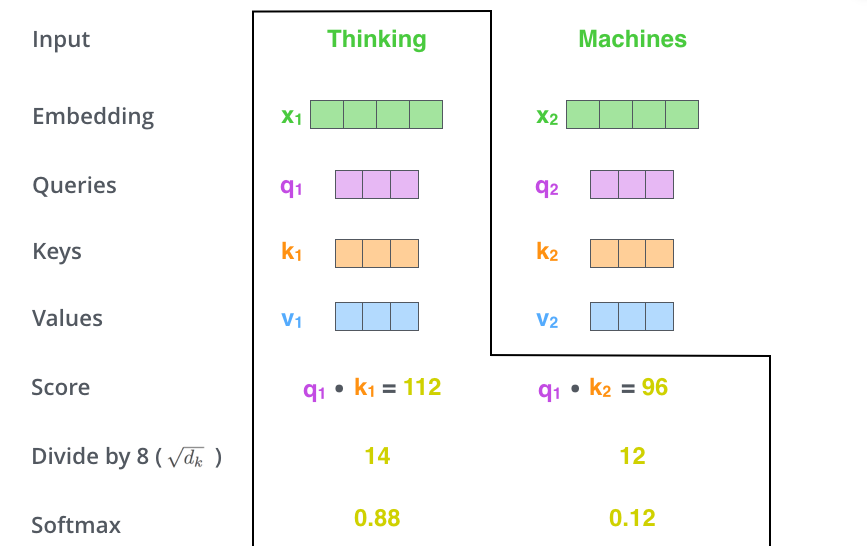
\includegraphics[width=0.8\linewidth]{step_3}
\end{frame}


\begin{frame}{Более детально}
\centering
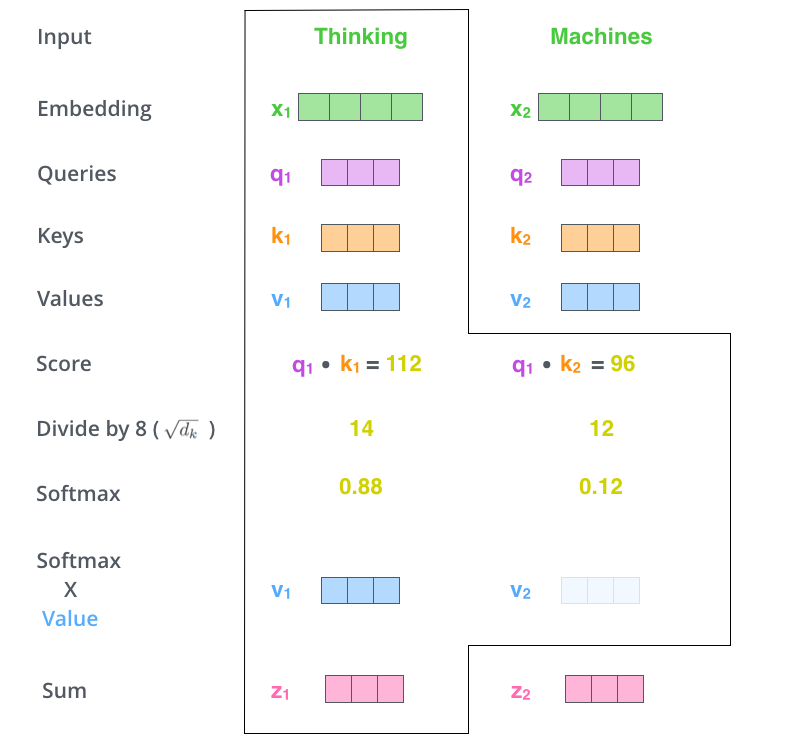
\includegraphics[width=0.5\linewidth]{step_4}
\end{frame}


\begin{frame}{Зверь с кучей голов} 
Несколько голов обеспечивают разное внимание
\begin{center}
	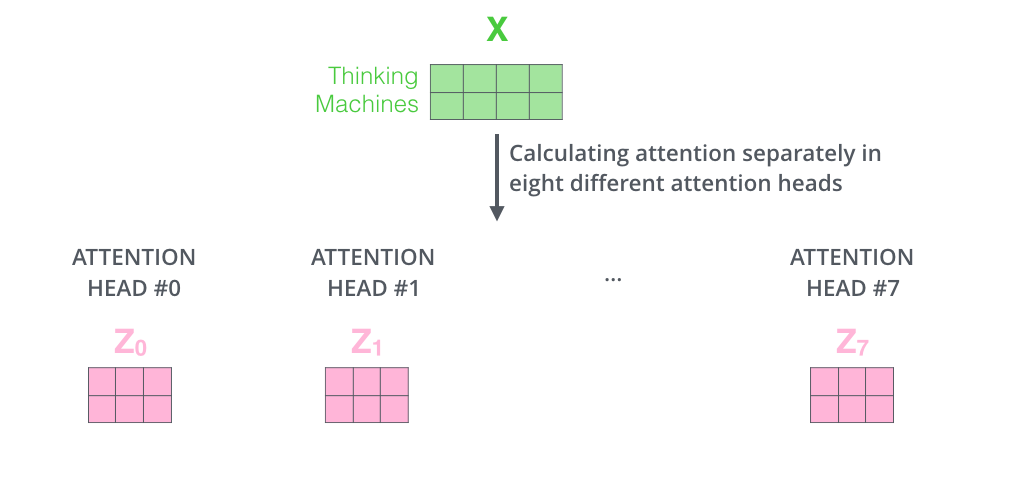
\includegraphics[width=.8\linewidth]{many_hads.png}
\end{center}
\end{frame}


\begin{frame}{Слой целиком} 
\begin{center}
	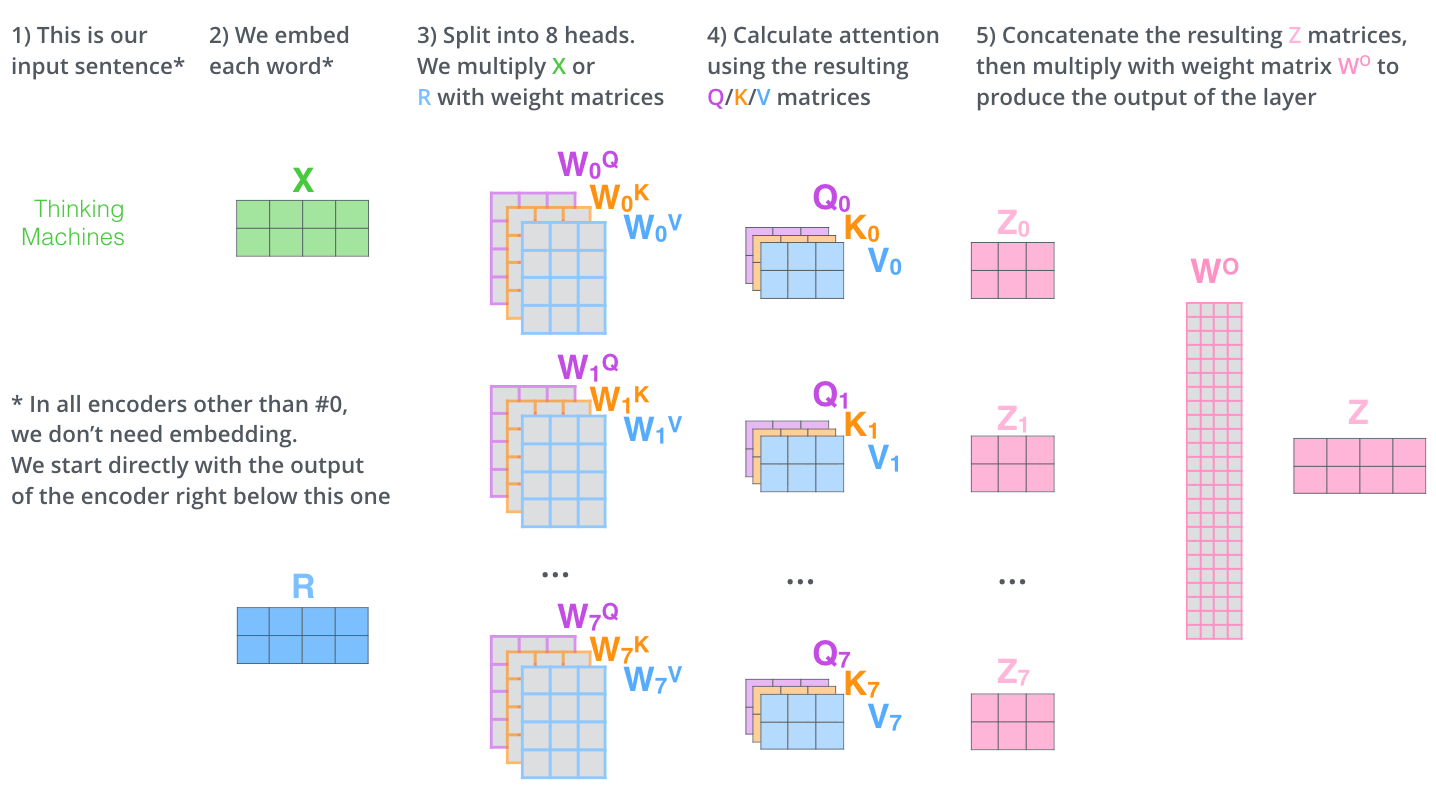
\includegraphics[width=.85\linewidth]{together.png}
\end{center}
\end{frame}


\begin{frame}{Positional encoding} 
Для учёта позиции слова в предложении входные эмбеддинги можно преобразовывать случайным шумом $t_i,$ который зависит от позиции (зашумлённый косинус и тп) 

\begin{center}
	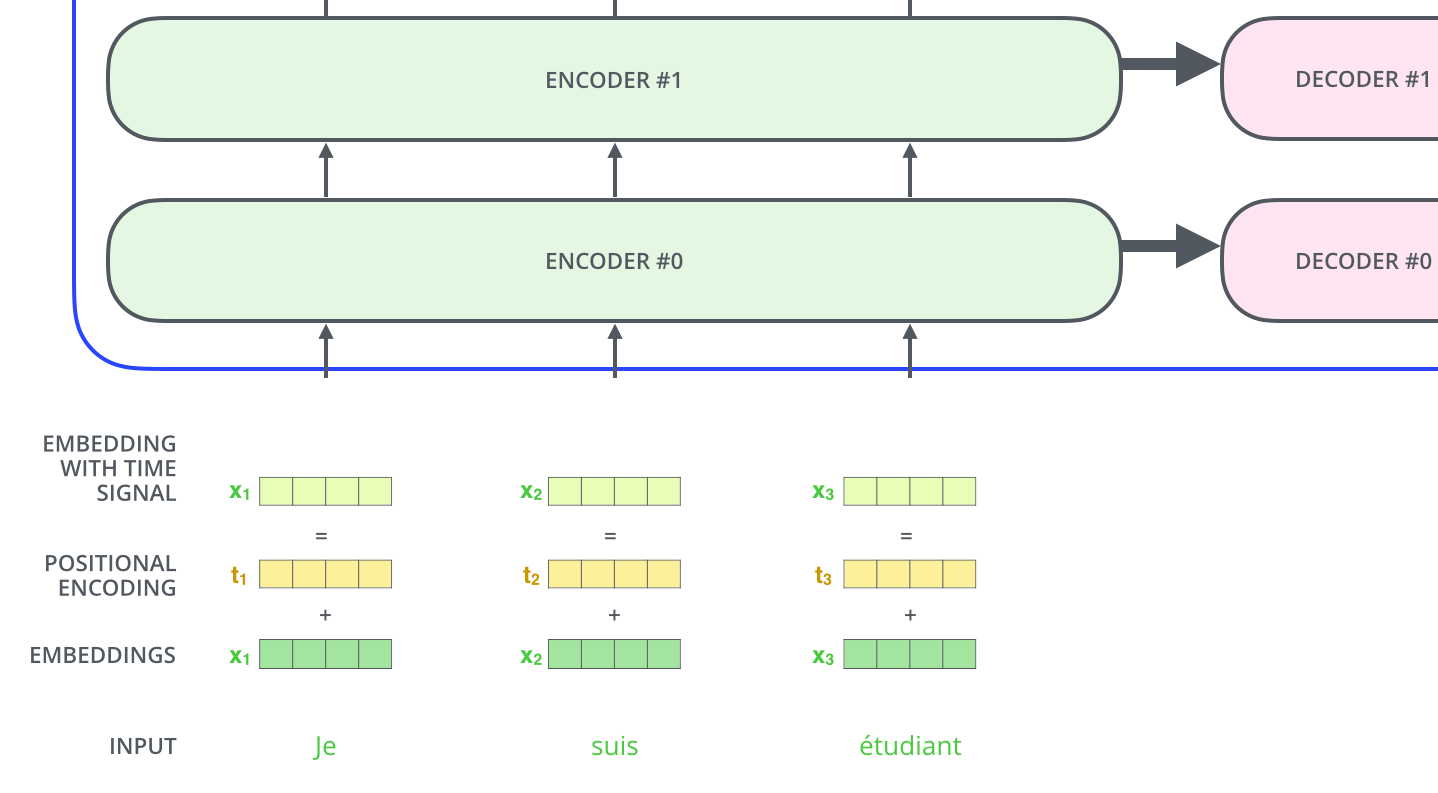
\includegraphics[width=.8\linewidth]{positional_encoding.png}
\end{center}
\end{frame}


\begin{frame}{Что происходит в декодере?} 
\begin{center}
	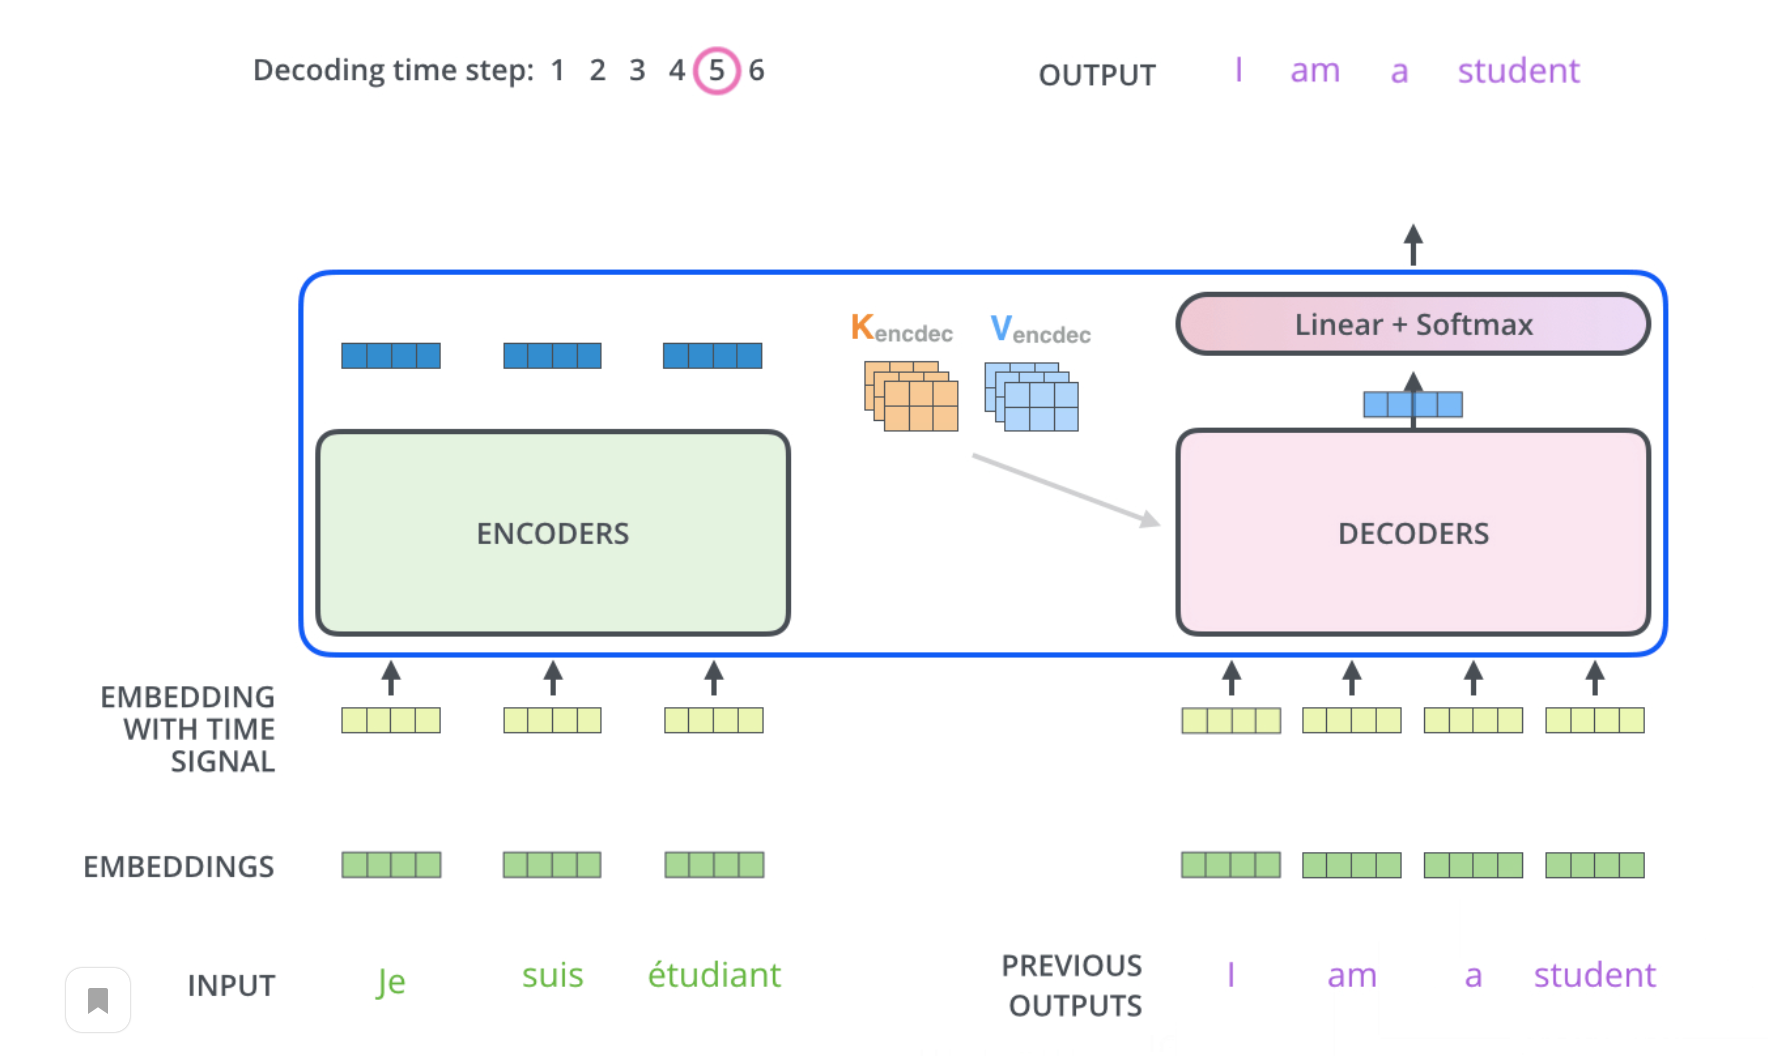
\includegraphics[width=.8\linewidth]{decoder.png}
\end{center}
\vfill
\footnotesize
{\color{blue} \url{http://jalammar.github.io/illustrated-transformer/}}
\end{frame}


\begin{transitionframe}
	\begin{center}
		\Huge Модификации трансформера
	\end{center}
\end{transitionframe}


\begin{frame}{Модификации}
\begin{wideitemize}
	\item  Большие объёмы неразмеченных данных в интернете в разных доменах (книги,
	новости, википедия, иные тексты из интернет-страниц)
	\item  Размеченных данных мало. Качественная разметка дорогая и долгая
	\item  Много вычислительных ресурсов, GPU, TPU, фреймворки распределённх
	вычислений
	\item Можем ли мы как-то заиспользовать имеющиеся ресурсы?
\end{wideitemize}
\end{frame}


\begin{frame}{Модификации}
\begin{wideitemize}
	\item  \alert{Да, можем! Использовать будем semi-supervised learning} 
	\item Обучаем большой трансформер на какой-нибудь unsupervised задаче на очень
	больших данных (очень долго, порядка нескольких недель на 64 гпу);
	\item Дообучаем трансформер на малом корпусе размеченных данных (очень быстро,
	порядка 1 часа на одной ГПУ).
\end{wideitemize}
\end{frame}


\begin{frame}{BERT (2018)}
\begin{center}
	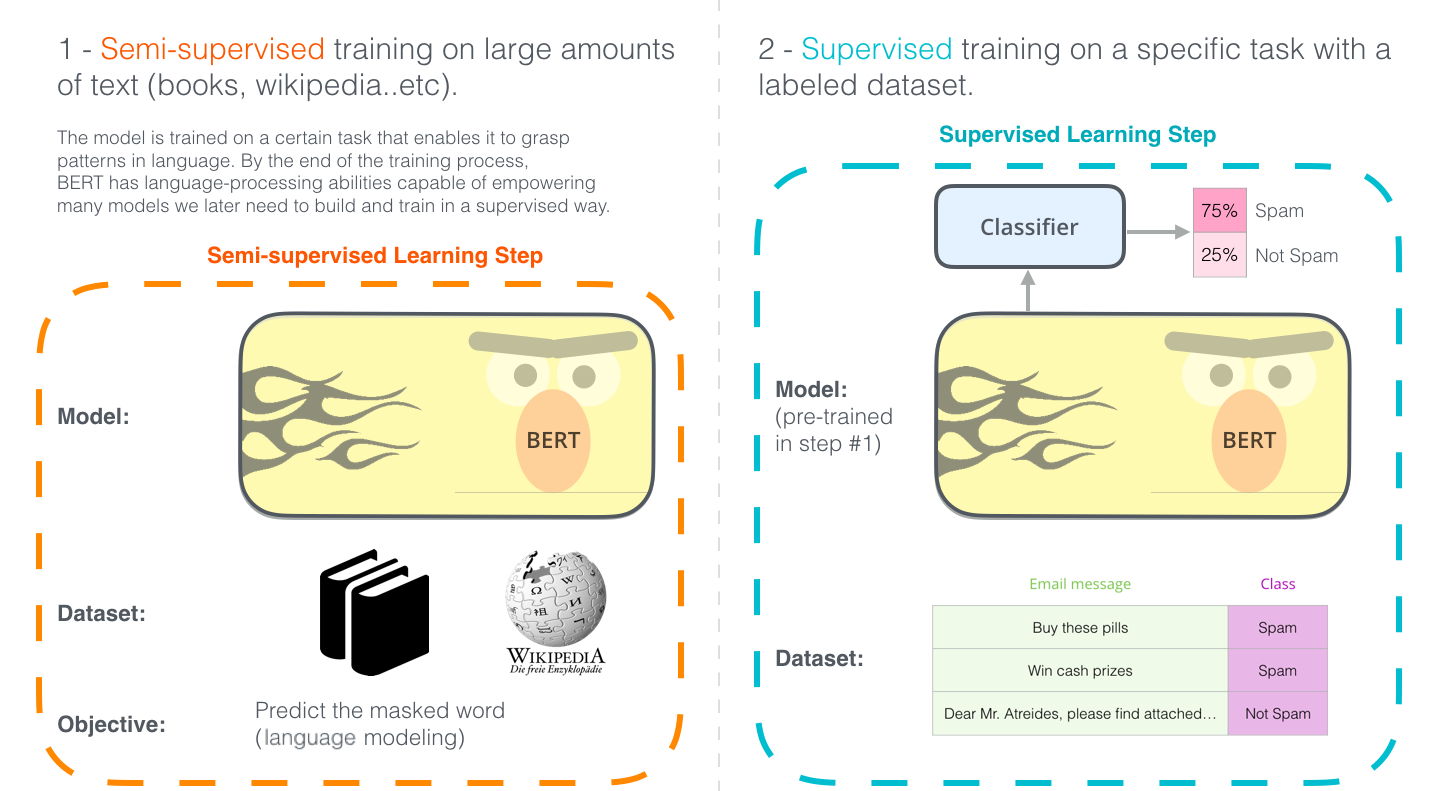
\includegraphics[width=0.8\linewidth]{BERT_stud}
\end{center}
\vfill
\footnotesize
{\color{blue} \url{http://jalammar.github.io/illustrated-bert/}}
\end{frame}


\begin{frame}{BERT (2018)}
\begin{center}
	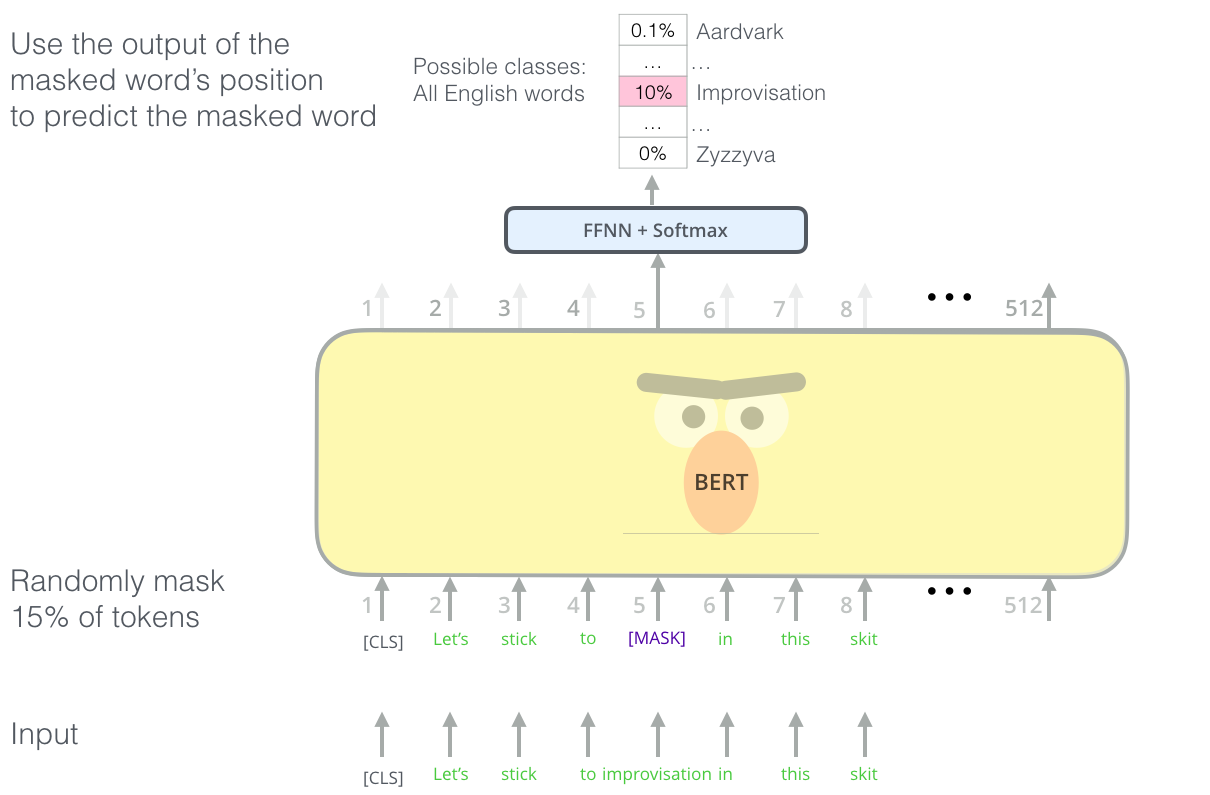
\includegraphics[width=0.7\linewidth]{pre_train_bert}
\end{center}
\vfill
\footnotesize
{\color{blue} \url{http://jalammar.github.io/illustrated-bert/}}
\end{frame}


\begin{frame}{BERT (2018)}
\begin{center}
	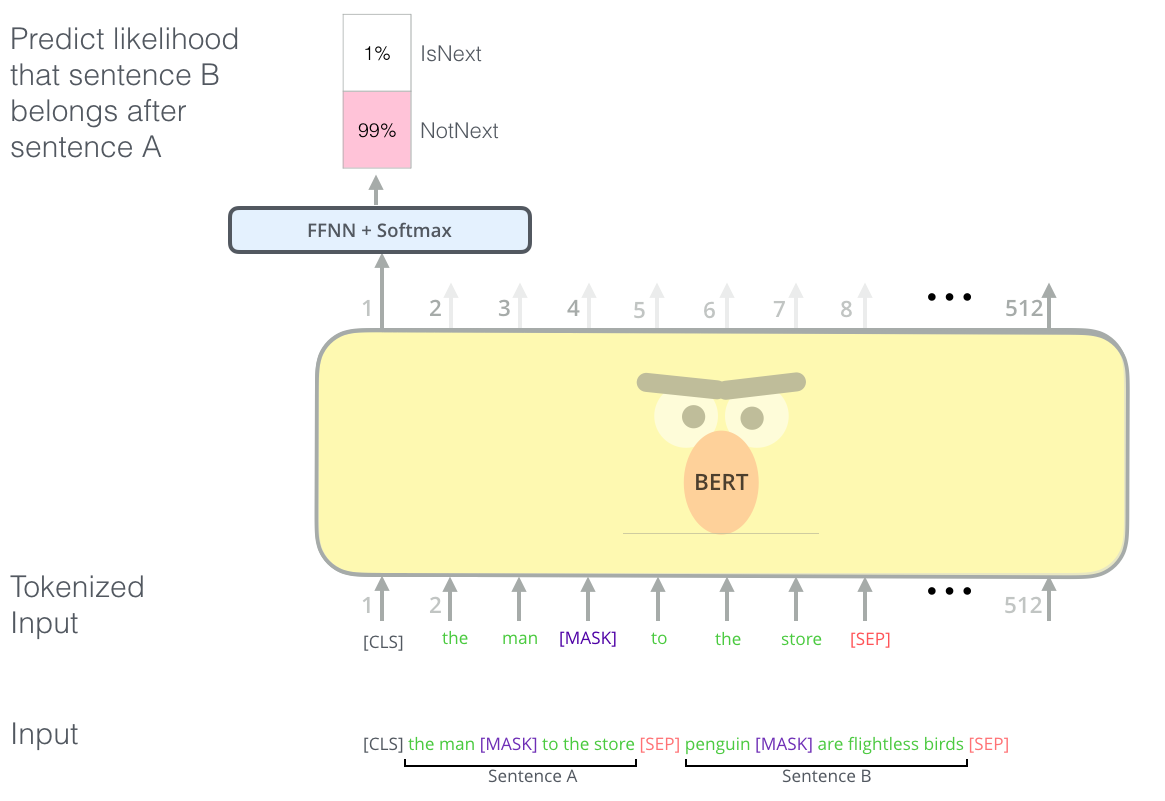
\includegraphics[width=0.65\linewidth]{bert_sent}
\end{center}
\vfill
\footnotesize
{\color{blue} \url{http://jalammar.github.io/illustrated-bert/}}
\end{frame}


\begin{frame}{BERT (2018)}
\begin{wideitemize}
	\item  BERT - Bidirectional Encoder Representations from Transformers
	\item  \alert{Идея BERT:} предобучать энкодер из трансформера на задаче Masked Language Modeling,
	\item А также на задаче Next Sentence Prediction
	\item После того, как мы предобучили BERT,  мы можем доучивать слои для решения конкретной задачи 
\end{wideitemize}
\end{frame}


\begin{frame}{Как используем?}
\begin{center}
	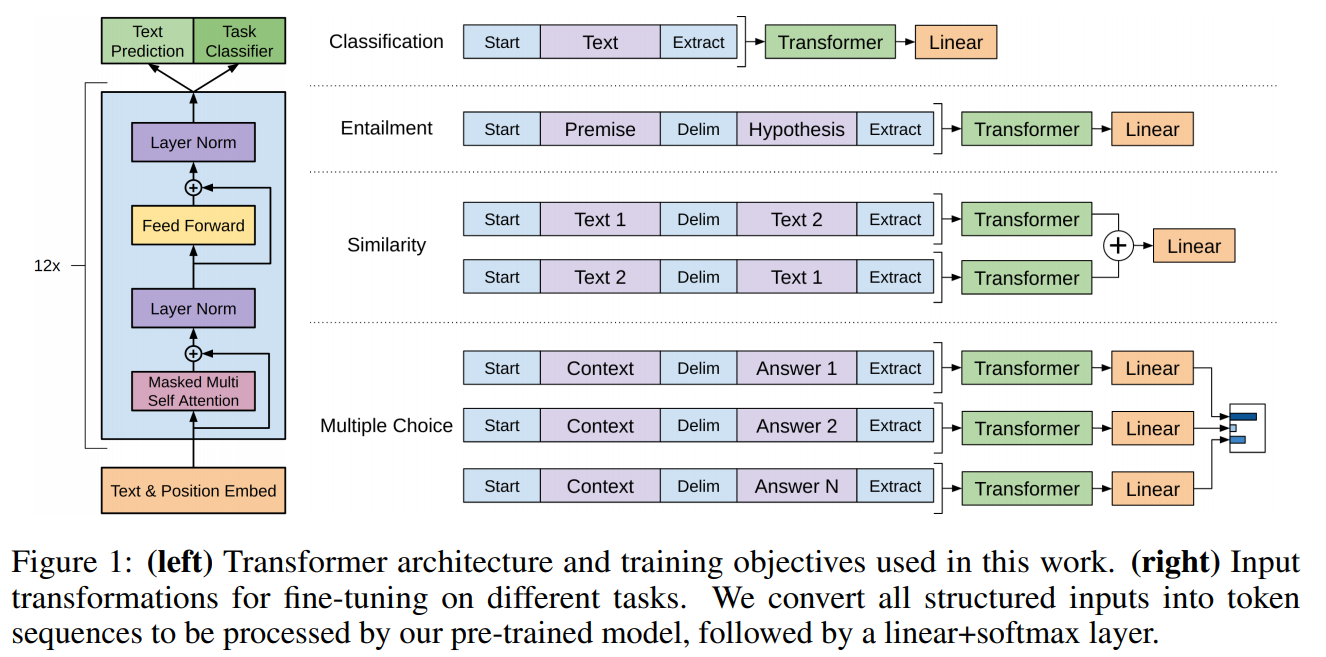
\includegraphics[width=0.9\linewidth]{images/use_models}
\end{center}
\end{frame}


%\begin{frame}{Итого}
%\begin{wideitemize}
%	\item У нас нет никаких слоев, кроме dense
%	\item Учится очень классно, находит множество взаимосвязей
%	\item \alert{Проблема:} огромный, каждый раз нужно прогонять текст через него
%	\item \alert{Решение:} 
%\end{wideitemize}
%\end{frame}


\end{document}
